
\chapter{Fonction logarithme décimal}
\competences{passer d'une écriture exponentielle à une écriture logarithmique, résoudre, modéliser}
\section{Cours de référence}
\begin{retenir}
Pour tout $b>0$, $\log(b)$ est l'unique réel $x$ tel que $10^x=b$. Ainsi $\log(10^x)=x$ et, pour $b>0$, $10^{\log(b)}=b$. La fonction $\log$ est définie sur $]0,+\infty[$ et elle est strictement croissante.
\end{retenir}

\begin{center}
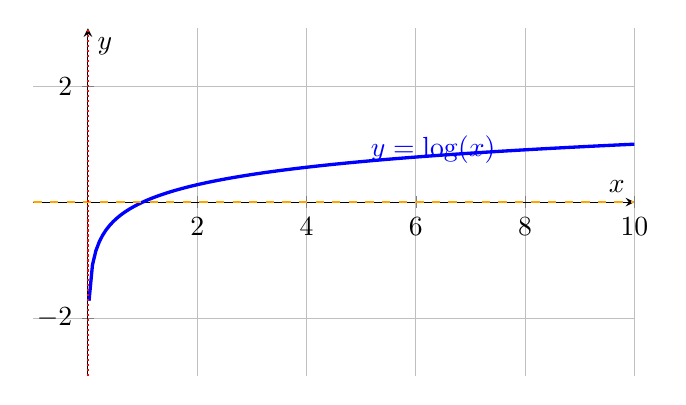
\begin{tikzpicture}
\begin{axis}[width=.76\textwidth,height=6cm,axis lines=middle,xmin=-1,xmax=10,ymin=-3,ymax=3,grid=major,xlabel={$x$},ylabel={$y$}]
\addplot[Blue,very thick,samples=160,domain=.02:10]{ln(x)/ln(10)};
\addplot[Orange,dashed,thick,domain=-1:10]{0};
\addplot[Red,densely dotted,thick] coordinates {(0,-3)(0,3)};
\node[anchor=west,Blue] at (axis cs:5,.9) {$y=\log(x)$};
\end{axis}
\end{tikzpicture}
\end{center}

Pour $a>0$, $b>0$ et tout entier naturel $n$ :
\[
\log(ab)=\log(a)+\log(b),\qquad
\log\!\left(\frac{a}{b}\right)=\log(a)-\log(b),\qquad
\log(a^n)=n\log(a).
\]

\begin{erreur}
$\log(a+b)$ ne se simplifie pas. Avant tout calcul logarithmique, vérifier que chaque argument est strictement positif.
\end{erreur}

\begin{methode}
Pour résoudre $a^x=b$, avec $a>0$, $a\neq1$ et $b>0$, on prend le logarithme : $x\log(a)=\log(b)$, donc $x=\dfrac{\log(b)}{\log(a)}$.
\end{methode}

\begin{exemple}
Résoudre $1{,}08^x=2$ revient à écrire $x=\dfrac{\log(2)}{\log(1{,}08)}\approx9{,}01$. Une valeur multipliée chaque année par $1{,}08$ double donc après un peu plus de neuf ans.
\end{exemple}

Comme $\log$ est croissante, pour $a,b>0$, $a<b$ équivaut à $\log(a)<\log(b)$. Pour $a>1$, $a^x<b$ équivaut à $x<\dfrac{\log b}{\log a}$ ; lorsque $0<a<1$, le sens de l'inégalité s'inverse.

\sessionheader{15}{17/11/2026}{B : 2 h -- C : 1 h}{Définition du logarithme décimal}{Fonction logarithme décimal}
\begin{objectifs}\begin{itemize}\item Relier puissance de 10 et logarithme.\item Calculer des valeurs usuelles.\item Utiliser la calculatrice.\end{itemize}\end{objectifs}
\begin{automatismes}\begin{enumerate}\item Calculer $20\,\%$ de $80$. \rep{$16$}\item Donner le domaine de $\log$. \rep{$]0,+\infty[$}\item Calculer $\log(10^4)$. \rep{$4$}\item Résoudre $10^x=0{,}01$. \rep{$x=-2$}\item Développer $\log(3b)$, $b>0$. \rep{$\log3+\log b$}\end{enumerate}\end{automatismes}
\begin{prerequis}Relire la dernière trace écrite et savoir effectuer les calculs élémentaires mobilisés aujourd'hui. Avant l'activité, faire reformuler les mots-clés : relier puissance de 10 et logarithme et calculer des valeurs usuelles.\end{prerequis}

\begin{activite}
Compléter les couples $10^x=b$ et $x=\log(b)$ pour $b=0{,}001;0{,}1;1;10;1\,000$. Puis utiliser la calculatrice pour $b=7$.

\end{activite}
\enseignant{Les logarithmes sont $-3,-1,0,1,3$ ; $\log(7)\approx0{,}8451$. Faire verbaliser la donnée qui déclenche le choix de méthode.}

\begin{traceecrite}Pour $b>0$, $\log(b)$ est l'unique solution de $10^x=b$. En particulier $\log(1)=0$, $\log(10)=1$ et $\log(100)=2$.\end{traceecrite}

\begin{exemple}
Reprendre les données de l'activité et rédiger la solution dans l'ordre : définition des objets, propriété utilisée, calcul exact ou approché, puis phrase de réponse. La réponse modèle figure dans l'édition enseignant.
\end{exemple}
\enseignant{Les logarithmes sont $-3,-1,0,1,3$ ; $\log(7)\approx0{,}8451$.}

\begin{exercice}[-- essentiel]
\begin{enumerate}\item Calculer $\log(10^2)$ et $\log(10^{-2})$.\item Développer $\log\!\left(\dfrac{100a^2}{b}\right)$ pour $a,b>0$.\item Résoudre $2^x=22$ et donner une valeur approchée au centième.\end{enumerate}
\end{exercice}
\enseignant{$2$ et $-2$. L'expression vaut $2+2\log(a)-\log(b)$. Enfin $x=\dfrac{\log(22)}{\log(2)}$.}

\manuelref{Calao, cours p. 64--69 ; exercices p. 70, n° 1 à 5}
\CalaoSession{15}

\begin{dm}Reprendre l'exercice d'entraînement 2 avec les données suivantes : remplacer la donnée initiale par $195$ et le taux ou la raison par $5$. Rédiger en quatre lignes : données, formule, calcul, conclusion.\end{dm}
\enseignant{La correction dépend de l'exercice repris. Vérifier surtout la cohérence du modèle, le nombre d'itérations, l'arrondi et la phrase de conclusion.}

\begin{sortie}Sur une demi-feuille : écrire la règle principale de la séance, traiter un exemple très court et indiquer son degré de confiance de 1 à 4. Question(s) essentielle(s) du jour : 1, 2 et 3.\end{sortie}

\ifprof
\begin{methode}
\textbf{Conduite en 1 h :} 7 min d'automatismes ; 10 min de mise en commun et trace ; 28 min d'exercices essentiels ; 5 min de correction ; 3 min de billet de sortie.\\
\textbf{Conduite en 2 h :} ajouter 20 min de recherche de l'activité, 20 min d'institutionnalisation, un second exercice autonome et 10 min de correction comparée.\\
\textbf{Différenciation :} fournir aux élèves fragiles une fiche à quatre cases (données, modèle, calcul, conclusion). Demander aux élèves rapides de produire un contre-exemple, une justification ou une seconde méthode.
\end{methode}
\fi
\sessionheader{16}{19/11/2026}{B : 1 h -- C : 2 h}{Sens de variation et représentation}{Fonction logarithme décimal}
\begin{objectifs}\begin{itemize}\item Connaître le domaine.\item Utiliser la croissance.\item Lire la courbe.\end{itemize}\end{objectifs}
\begin{automatismes}\begin{enumerate}\item Écrire le coefficient multiplicateur d'une hausse de $25\,\%$. \rep{$1+\dfrac{25}{100}=1,25$}\item Calculer $\log(10^0)$. \rep{$0$}\item Résoudre $10^x=0{,}01$. \rep{$x=-2$}\item Développer $\log(3b)$, $b>0$. \rep{$\log3+\log b$}\item Donner le domaine de $\log$. \rep{$]0,+\infty[$}\end{enumerate}\end{automatismes}
\begin{prerequis}Relire la dernière trace écrite et savoir effectuer les calculs élémentaires mobilisés aujourd'hui. Avant l'activité, faire reformuler les mots-clés : connaître le domaine et utiliser la croissance.\end{prerequis}

\begin{activite}
Tracer $y=10^x$ et la droite $y=x$, puis obtenir la courbe du logarithme par symétrie. En déduire son domaine, son sens de variation et l'asymptote.
\begin{center}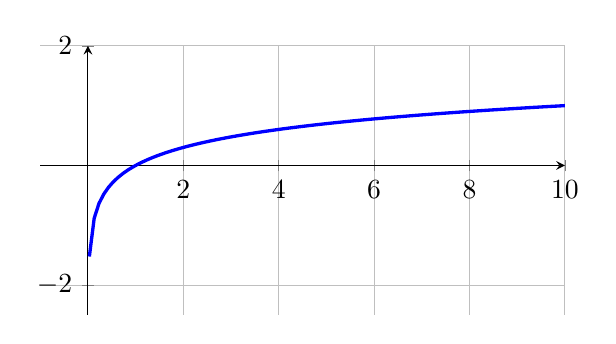
\begin{tikzpicture}\begin{axis}[width=.68\textwidth,height=5cm,axis lines=middle,xmin=-1,xmax=10,ymin=-2.5,ymax=2,grid=major]\addplot[Blue,very thick,samples=100,domain=.03:10]{ln(x)/ln(10)};\end{axis}\end{tikzpicture}\end{center}
\end{activite}
\enseignant{Le logarithme est la fonction réciproque de $10^x$ : domaine $]0,+\infty[$, croissance stricte, asymptote $x=0$. Faire verbaliser la donnée qui déclenche le choix de méthode.}

\begin{traceecrite}La fonction $\log$ est définie sur $]0,+\infty[$, strictement croissante, et sa courbe admet $x=0$ comme asymptote verticale.\end{traceecrite}

\begin{exemple}
Reprendre les données de l'activité et rédiger la solution dans l'ordre : définition des objets, propriété utilisée, calcul exact ou approché, puis phrase de réponse. La réponse modèle figure dans l'édition enseignant.
\end{exemple}
\enseignant{Le logarithme est la fonction réciproque de $10^x$ : domaine $]0,+\infty[$, croissance stricte, asymptote $x=0$.}

\begin{exercice}[-- essentiel]
\begin{enumerate}\item Calculer $\log(10^3)$ et $\log(10^{-3})$.\item Développer $\log\!\left(\dfrac{100a^2}{b}\right)$ pour $a,b>0$.\item Résoudre $3^x=23$ et donner une valeur approchée au centième.\end{enumerate}
\end{exercice}
\enseignant{$3$ et $-3$. L'expression vaut $2+2\log(a)-\log(b)$. Enfin $x=\dfrac{\log(23)}{\log(3)}$.}

\manuelref{Calao, cours p. 64--69 ; exercices p. 70, n° 6 à 10}
\CalaoSession{16}

\begin{dm}Reprendre l'exercice d'entraînement 3 avec les données suivantes : remplacer la donnée initiale par $200$ et le taux ou la raison par $6$. Rédiger en quatre lignes : données, formule, calcul, conclusion.\end{dm}
\enseignant{La correction dépend de l'exercice repris. Vérifier surtout la cohérence du modèle, le nombre d'itérations, l'arrondi et la phrase de conclusion.}

\begin{sortie}Sur une demi-feuille : écrire la règle principale de la séance, traiter un exemple très court et indiquer son degré de confiance de 1 à 4. Question(s) essentielle(s) du jour : 1 et 2.\end{sortie}

\ifprof
\begin{methode}
\textbf{Conduite en 1 h :} 7 min d'automatismes ; 10 min de mise en commun et trace ; 28 min d'exercices essentiels ; 5 min de correction ; 3 min de billet de sortie.\\
\textbf{Conduite en 2 h :} ajouter 20 min de recherche de l'activité, 20 min d'institutionnalisation, un second exercice autonome et 10 min de correction comparée.\\
\textbf{Différenciation :} fournir aux élèves fragiles une fiche à quatre cases (données, modèle, calcul, conclusion). Demander aux élèves rapides de produire un contre-exemple, une justification ou une seconde méthode.
\end{methode}
\fi
\sessionheader{17}{24/11/2026}{B : 2 h -- C : 1 h}{Propriétés algébriques}{Fonction logarithme décimal}
\begin{objectifs}\begin{itemize}\item Développer ou condenser des logarithmes.\item Vérifier les conditions.\item Éviter les fausses propriétés.\end{itemize}\end{objectifs}
\begin{automatismes}\begin{enumerate}\item Réduire $3x+6-x+2$. \rep{$2x+8$}\item Résoudre $10^x=0{,}01$. \rep{$x=-2$}\item Développer $\log(3b)$, $b>0$. \rep{$\log3+\log b$}\item Donner le domaine de $\log$. \rep{$]0,+\infty[$}\item Calculer $\log(10^1)$. \rep{$1$}\end{enumerate}\end{automatismes}
\begin{prerequis}Relire la dernière trace écrite et savoir effectuer les calculs élémentaires mobilisés aujourd'hui. Avant l'activité, faire reformuler les mots-clés : développer ou condenser des logarithmes et vérifier les conditions.\end{prerequis}

\begin{activite}
À partir de $10^2\times10^3=10^5$, conjecturer $\log(ab)=\log a+\log b$. Tester numériquement avec $a=2,b=5$, puis expliquer pourquoi $a,b$ doivent être positifs.

\end{activite}
\enseignant{$\log(2)+\log(5)=\log(10)=1$. Le logarithme n'est défini que pour un argument strictement positif. Faire verbaliser la donnée qui déclenche le choix de méthode.}

\begin{traceecrite}Pour $a,b>0$, $\log(ab)=\log a+\log b$ et $\log\!\left(\dfrac ab\right)=\log a-\log b$. De plus $\log(a^n)=n\log a$.\end{traceecrite}

\begin{exemple}
Reprendre les données de l'activité et rédiger la solution dans l'ordre : définition des objets, propriété utilisée, calcul exact ou approché, puis phrase de réponse. La réponse modèle figure dans l'édition enseignant.
\end{exemple}
\enseignant{$\log(2)+\log(5)=\log(10)=1$. Le logarithme n'est défini que pour un argument strictement positif.}

\begin{exercice}[-- essentiel]
\begin{enumerate}\item Calculer $\log(10^4)$ et $\log(10^{-4})$.\item Développer $\log\!\left(\dfrac{100a^2}{b}\right)$ pour $a,b>0$.\item Résoudre $4^x=24$ et donner une valeur approchée au centième.\end{enumerate}
\end{exercice}
\enseignant{$4$ et $-4$. L'expression vaut $2+2\log(a)-\log(b)$. Enfin $x=\dfrac{\log(24)}{\log(4)}$.}

\manuelref{Calao, cours p. 66--69 ; exercices p. 72, n° 20 à 23}
\CalaoSession{17}

\begin{dm}Reprendre l'exercice d'entraînement 2 avec les données suivantes : remplacer la donnée initiale par $205$ et le taux ou la raison par $7$. Rédiger en quatre lignes : données, formule, calcul, conclusion.\end{dm}
\enseignant{La correction dépend de l'exercice repris. Vérifier surtout la cohérence du modèle, le nombre d'itérations, l'arrondi et la phrase de conclusion.}

\begin{sortie}Sur une demi-feuille : écrire la règle principale de la séance, traiter un exemple très court et indiquer son degré de confiance de 1 à 4. Question(s) essentielle(s) du jour : 1, 2 et 3.\end{sortie}

\ifprof
\begin{methode}
\textbf{Conduite en 1 h :} 7 min d'automatismes ; 10 min de mise en commun et trace ; 28 min d'exercices essentiels ; 5 min de correction ; 3 min de billet de sortie.\\
\textbf{Conduite en 2 h :} ajouter 20 min de recherche de l'activité, 20 min d'institutionnalisation, un second exercice autonome et 10 min de correction comparée.\\
\textbf{Différenciation :} fournir aux élèves fragiles une fiche à quatre cases (données, modèle, calcul, conclusion). Demander aux élèves rapides de produire un contre-exemple, une justification ou une seconde méthode.
\end{methode}
\fi
\sessionheader{18}{26/11/2026}{B : 1 h -- C : 2 h}{Résoudre $10^x=b$}{Fonction logarithme décimal}
\begin{objectifs}\begin{itemize}\item Résoudre $10^x=b$.\item Encadrer une solution.\item Interpréter un ordre de grandeur.\end{itemize}\end{objectifs}
\begin{automatismes}\begin{enumerate}\item Calculer $5\,\%$ de $140$. \rep{$7$}\item Développer $\log(3b)$, $b>0$. \rep{$\log3+\log b$}\item Donner le domaine de $\log$. \rep{$]0,+\infty[$}\item Calculer $\log(10^2)$. \rep{$2$}\item Résoudre $10^x=0{,}01$. \rep{$x=-2$}\end{enumerate}\end{automatismes}
\begin{prerequis}Relire la dernière trace écrite et savoir effectuer les calculs élémentaires mobilisés aujourd'hui. Avant l'activité, faire reformuler les mots-clés : résoudre $10^x=b$ et encadrer une solution.\end{prerequis}

\begin{activite}
Un appareil mesure des intensités $b=0{,}04;3{,}2;850$. Pour chaque valeur, résoudre $10^x=b$, donner $x$ au centième et vérifier en calculant $10^x$.

\end{activite}
\enseignant{$x=\log(b)$ : environ $-1{,}40$, $0{,}51$ et $2{,}93$. Faire verbaliser la donnée qui déclenche le choix de méthode.}

\begin{traceecrite}L'équation $10^x=b$ n'a de solution que si $b>0$ ; cette solution est $x=\log(b)$.\end{traceecrite}

\begin{exemple}
Reprendre les données de l'activité et rédiger la solution dans l'ordre : définition des objets, propriété utilisée, calcul exact ou approché, puis phrase de réponse. La réponse modèle figure dans l'édition enseignant.
\end{exemple}
\enseignant{$x=\log(b)$ : environ $-1{,}40$, $0{,}51$ et $2{,}93$.}

\begin{exercice}[-- essentiel]
\begin{enumerate}\item Calculer $\log(10^5)$ et $\log(10^{-5})$.\item Développer $\log\!\left(\dfrac{100a^2}{b}\right)$ pour $a,b>0$.\item Résoudre $5^x=25$ et donner une valeur approchée au centième.\end{enumerate}
\end{exercice}
\enseignant{$5$ et $-5$. L'expression vaut $2+2\log(a)-\log(b)$. Enfin $x=\dfrac{\log(25)}{\log(5)}$.}

\manuelref{Calao, p. 73, n° 30 à 32}
\CalaoSession{18}

\begin{dm}Reprendre l'exercice d'entraînement 3 avec les données suivantes : remplacer la donnée initiale par $210$ et le taux ou la raison par $2$. Rédiger en quatre lignes : données, formule, calcul, conclusion.\end{dm}
\enseignant{La correction dépend de l'exercice repris. Vérifier surtout la cohérence du modèle, le nombre d'itérations, l'arrondi et la phrase de conclusion.}

\begin{sortie}Sur une demi-feuille : écrire la règle principale de la séance, traiter un exemple très court et indiquer son degré de confiance de 1 à 4. Question(s) essentielle(s) du jour : 1 et 2.\end{sortie}

\ifprof
\begin{methode}
\textbf{Conduite en 1 h :} 7 min d'automatismes ; 10 min de mise en commun et trace ; 28 min d'exercices essentiels ; 5 min de correction ; 3 min de billet de sortie.\\
\textbf{Conduite en 2 h :} ajouter 20 min de recherche de l'activité, 20 min d'institutionnalisation, un second exercice autonome et 10 min de correction comparée.\\
\textbf{Différenciation :} fournir aux élèves fragiles une fiche à quatre cases (données, modèle, calcul, conclusion). Demander aux élèves rapides de produire un contre-exemple, une justification ou une seconde méthode.
\end{methode}
\fi
\sessionheader{19}{01/12/2026}{B : 2 h -- C : 1 h}{Résoudre $a^x=b$}{Fonction logarithme décimal}
\begin{objectifs}\begin{itemize}\item Résoudre $a^x=b$.\item Utiliser un quotient de logarithmes.\item Arrondir avec sens.\end{itemize}\end{objectifs}
\begin{automatismes}\begin{enumerate}\item Écrire le coefficient multiplicateur d'une hausse de $10\,\%$. \rep{$1+\dfrac{10}{100}=1,10$}\item Donner le domaine de $\log$. \rep{$]0,+\infty[$}\item Calculer $\log(10^3)$. \rep{$3$}\item Résoudre $10^x=0{,}01$. \rep{$x=-2$}\item Développer $\log(3b)$, $b>0$. \rep{$\log3+\log b$}\end{enumerate}\end{automatismes}
\begin{prerequis}Relire la dernière trace écrite et savoir effectuer les calculs élémentaires mobilisés aujourd'hui. Avant l'activité, faire reformuler les mots-clés : résoudre $a^x=b$ et utiliser un quotient de logarithmes.\end{prerequis}

\begin{activite}
Le nombre d'abonnés est multiplié par $1{,}15$ chaque mois. Déterminer au bout de combien de mois il aura triplé. Poser l'équation, la résoudre avec les logarithmes et interpréter l'arrondi.

\end{activite}
\enseignant{$1{,}15^n\geq3$ ; $\dfrac{\log3}{\log1{,}15}\approx7{,}86$. Il faut donc huit mois entiers. Faire verbaliser la donnée qui déclenche le choix de méthode.}

\begin{traceecrite}Pour $a>0$, $a\neq1$ et $b>0$, $a^x=b$ équivaut à $x=\dfrac{\log(b)}{\log(a)}$.\end{traceecrite}

\begin{exemple}
Reprendre les données de l'activité et rédiger la solution dans l'ordre : définition des objets, propriété utilisée, calcul exact ou approché, puis phrase de réponse. La réponse modèle figure dans l'édition enseignant.
\end{exemple}
\enseignant{$1{,}15^n\geq3$ ; $\dfrac{\log3}{\log1{,}15}\approx7{,}86$. Il faut donc huit mois entiers.}

\begin{exercice}[-- essentiel]
\begin{enumerate}\item Calculer $\log(10^6)$ et $\log(10^{-6})$.\item Développer $\log\!\left(\dfrac{100a^2}{b}\right)$ pour $a,b>0$.\item Résoudre $6^x=26$ et donner une valeur approchée au centième.\end{enumerate}
\end{exercice}
\enseignant{$6$ et $-6$. L'expression vaut $2+2\log(a)-\log(b)$. Enfin $x=\dfrac{\log(26)}{\log(6)}$.}

\manuelref{Calao, p. 74, n° 33 à 39}
\CalaoSession{19}

\begin{dm}Reprendre l'exercice d'entraînement 2 avec les données suivantes : remplacer la donnée initiale par $215$ et le taux ou la raison par $3$. Rédiger en quatre lignes : données, formule, calcul, conclusion.\end{dm}
\enseignant{La correction dépend de l'exercice repris. Vérifier surtout la cohérence du modèle, le nombre d'itérations, l'arrondi et la phrase de conclusion.}

\begin{sortie}Sur une demi-feuille : écrire la règle principale de la séance, traiter un exemple très court et indiquer son degré de confiance de 1 à 4. Question(s) essentielle(s) du jour : 1, 2 et 3.\end{sortie}

\ifprof
\begin{methode}
\textbf{Conduite en 1 h :} 7 min d'automatismes ; 10 min de mise en commun et trace ; 28 min d'exercices essentiels ; 5 min de correction ; 3 min de billet de sortie.\\
\textbf{Conduite en 2 h :} ajouter 20 min de recherche de l'activité, 20 min d'institutionnalisation, un second exercice autonome et 10 min de correction comparée.\\
\textbf{Différenciation :} fournir aux élèves fragiles une fiche à quatre cases (données, modèle, calcul, conclusion). Demander aux élèves rapides de produire un contre-exemple, une justification ou une seconde méthode.
\end{methode}
\fi
\sessionheader{20}{03/12/2026}{B : 1 h -- C : 2 h}{Équations $x^a=b$ et inégalités simples}{Fonction logarithme décimal}
\begin{objectifs}\begin{itemize}\item Résoudre une puissance inconnue.\item Traiter une inégalité.\item Tenir compte du domaine.\end{itemize}\end{objectifs}
\begin{automatismes}\begin{enumerate}\item Réduire $3x+9-x+2$. \rep{$2x+11$}\item Calculer $\log(10^4)$. \rep{$4$}\item Résoudre $10^x=0{,}01$. \rep{$x=-2$}\item Développer $\log(3b)$, $b>0$. \rep{$\log3+\log b$}\item Donner le domaine de $\log$. \rep{$]0,+\infty[$}\end{enumerate}\end{automatismes}
\begin{prerequis}Relire la dernière trace écrite et savoir effectuer les calculs élémentaires mobilisés aujourd'hui. Avant l'activité, faire reformuler les mots-clés : résoudre une puissance inconnue et traiter une inégalité.\end{prerequis}

\begin{activite}
Résoudre sur $[0,+\infty[$ : $x^3=40$, puis $x^4=16$. Résoudre ensuite $1{,}08^x<1{,}5$ et expliquer le rôle de la croissance.

\end{activite}
\enseignant{$x=\sqrt[3]{40}\approx3{,}42$ ; $x=2$ sur l'intervalle demandé ; $x<\dfrac{\log1{,}5}{\log1{,}08}\approx5{,}27$. Faire verbaliser la donnée qui déclenche le choix de méthode.}

\begin{traceecrite}Pour résoudre $x^n=b$, tenir compte du domaine et de la parité de $n$. Pour une inégalité exponentielle, le sens dépend de la croissance ou décroissance de la fonction.\end{traceecrite}

\begin{exemple}
Reprendre les données de l'activité et rédiger la solution dans l'ordre : définition des objets, propriété utilisée, calcul exact ou approché, puis phrase de réponse. La réponse modèle figure dans l'édition enseignant.
\end{exemple}
\enseignant{$x=\sqrt[3]{40}\approx3{,}42$ ; $x=2$ sur l'intervalle demandé ; $x<\dfrac{\log1{,}5}{\log1{,}08}\approx5{,}27$.}

\begin{exercice}[-- essentiel]
\begin{enumerate}\item Calculer $\log(10^2)$ et $\log(10^{-2})$.\item Développer $\log\!\left(\dfrac{100a^2}{b}\right)$ pour $a,b>0$.\item Résoudre $2^x=22$ et donner une valeur approchée au centième.\end{enumerate}
\end{exercice}
\enseignant{$2$ et $-2$. L'expression vaut $2+2\log(a)-\log(b)$. Enfin $x=\dfrac{\log(22)}{\log(2)}$.}

\manuelref{Calao, p. 75, n° 40 à 42}
\CalaoSession{20}

\begin{dm}Reprendre l'exercice d'entraînement 3 avec les données suivantes : remplacer la donnée initiale par $220$ et le taux ou la raison par $4$. Rédiger en quatre lignes : données, formule, calcul, conclusion.\end{dm}
\enseignant{La correction dépend de l'exercice repris. Vérifier surtout la cohérence du modèle, le nombre d'itérations, l'arrondi et la phrase de conclusion.}

\begin{sortie}Sur une demi-feuille : écrire la règle principale de la séance, traiter un exemple très court et indiquer son degré de confiance de 1 à 4. Question(s) essentielle(s) du jour : 1 et 2.\end{sortie}

\ifprof
\begin{methode}
\textbf{Conduite en 1 h :} 7 min d'automatismes ; 10 min de mise en commun et trace ; 28 min d'exercices essentiels ; 5 min de correction ; 3 min de billet de sortie.\\
\textbf{Conduite en 2 h :} ajouter 20 min de recherche de l'activité, 20 min d'institutionnalisation, un second exercice autonome et 10 min de correction comparée.\\
\textbf{Différenciation :} fournir aux élèves fragiles une fiche à quatre cases (données, modèle, calcul, conclusion). Demander aux élèves rapides de produire un contre-exemple, une justification ou une seconde méthode.
\end{methode}
\fi
\sessionheader{21}{08/12/2026}{B : 2 h -- C : 1 h}{Problèmes contextualisés}{Fonction logarithme décimal}
\begin{objectifs}\begin{itemize}\item Modéliser une situation.\item Choisir une équation.\item Conclure dans le contexte.\end{itemize}\end{objectifs}
\begin{automatismes}\begin{enumerate}\item Calculer $20\,\%$ de $60$. \rep{$12$}\item Résoudre $10^x=0{,}01$. \rep{$x=-2$}\item Développer $\log(3b)$, $b>0$. \rep{$\log3+\log b$}\item Donner le domaine de $\log$. \rep{$]0,+\infty[$}\item Calculer $\log(10^3)$. \rep{$3$}\end{enumerate}\end{automatismes}
\begin{prerequis}Relire la dernière trace écrite et savoir effectuer les calculs élémentaires mobilisés aujourd'hui. Avant l'activité, faire reformuler les mots-clés : modéliser une situation et choisir une équation.\end{prerequis}

\begin{activite}
Le niveau sonore est $L=10\log\!\left(\dfrac I{I_0}\right)$. Calculer $L$ lorsque $I=10^6I_0$. Puis déterminer le rapport $\dfrac I{I_0}$ pour $L=85$ dB.

\end{activite}
\enseignant{$L=60$ dB. Pour $85$ dB, $\log\!\left(\dfrac I{I_0}\right)=8{,}5$, donc $\dfrac I{I_0}=10^{8{,}5}\approx3{,}16\times10^8$. Faire verbaliser la donnée qui déclenche le choix de méthode.}

\begin{traceecrite}Dans un problème, définir la variable, poser l'équation, résoudre, contrôler le domaine et conclure avec l'unité. Une solution numérique sans interprétation est incomplète.\end{traceecrite}

\begin{exemple}
Reprendre les données de l'activité et rédiger la solution dans l'ordre : définition des objets, propriété utilisée, calcul exact ou approché, puis phrase de réponse. La réponse modèle figure dans l'édition enseignant.
\end{exemple}
\enseignant{$L=60$ dB. Pour $85$ dB, $\log\!\left(\dfrac I{I_0}\right)=8{,}5$, donc $\dfrac I{I_0}=10^{8{,}5}\approx3{,}16\times10^8$.}

\begin{exercice}[-- essentiel]
\begin{enumerate}\item Calculer $\log(10^3)$ et $\log(10^{-3})$.\item Développer $\log\!\left(\dfrac{100a^2}{b}\right)$ pour $a,b>0$.\item Résoudre $3^x=23$ et donner une valeur approchée au centième.\end{enumerate}
\end{exercice}
\enseignant{$3$ et $-3$. L'expression vaut $2+2\log(a)-\log(b)$. Enfin $x=\dfrac{\log(23)}{\log(3)}$.}

\manuelref{Calao, p. 74, n° 38--39, puis p. 75, n° 40 à 42}
\CalaoSession{21}

\begin{dm}Reprendre l'exercice d'entraînement 2 avec les données suivantes : remplacer la donnée initiale par $225$ et le taux ou la raison par $5$. Rédiger en quatre lignes : données, formule, calcul, conclusion.\end{dm}
\enseignant{La correction dépend de l'exercice repris. Vérifier surtout la cohérence du modèle, le nombre d'itérations, l'arrondi et la phrase de conclusion.}

\begin{sortie}Sur une demi-feuille : écrire la règle principale de la séance, traiter un exemple très court et indiquer son degré de confiance de 1 à 4. Question(s) essentielle(s) du jour : 1, 2 et 3.\end{sortie}

\ifprof
\begin{methode}
\textbf{Conduite en 1 h :} 7 min d'automatismes ; 10 min de mise en commun et trace ; 28 min d'exercices essentiels ; 5 min de correction ; 3 min de billet de sortie.\\
\textbf{Conduite en 2 h :} ajouter 20 min de recherche de l'activité, 20 min d'institutionnalisation, un second exercice autonome et 10 min de correction comparée.\\
\textbf{Différenciation :} fournir aux élèves fragiles une fiche à quatre cases (données, modèle, calcul, conclusion). Demander aux élèves rapides de produire un contre-exemple, une justification ou une seconde méthode.
\end{methode}
\fi
\sessionheader{22}{10/12/2026}{B : 1 h -- C : 2 h}{Bilan et évaluation}{Fonction logarithme décimal}
\begin{objectifs}\begin{itemize}\item Synthétiser les méthodes.\item Identifier les conditions.\item Remédier aux erreurs.\end{itemize}\end{objectifs}
\begin{automatismes}\begin{enumerate}\item Écrire le coefficient multiplicateur d'une hausse de $25\,\%$. \rep{$1+\dfrac{25}{100}=1,25$}\item Développer $\log(3b)$, $b>0$. \rep{$\log3+\log b$}\item Donner le domaine de $\log$. \rep{$]0,+\infty[$}\item Calculer $\log(10^4)$. \rep{$4$}\item Résoudre $10^x=0{,}01$. \rep{$x=-2$}\end{enumerate}\end{automatismes}
\begin{prerequis}Relire la dernière trace écrite et savoir effectuer les calculs élémentaires mobilisés aujourd'hui. Avant l'activité, faire reformuler les mots-clés : synthétiser les méthodes et identifier les conditions.\end{prerequis}

\begin{activite}
Réaliser une carte de méthodes : domaine ; propriétés ; équations $10^x=b$ ; équations $a^x=b$ ; inégalités. Associer à chaque branche une condition et un exemple.

\end{activite}
\enseignant{La carte doit notamment faire apparaître la positivité des arguments et la distinction entre base supérieure à $1$ ou comprise entre $0$ et $1$. Faire verbaliser la donnée qui déclenche le choix de méthode.}

\begin{traceecrite}Avant un calcul de logarithme : vérifier la positivité. Avant une comparaison : identifier le sens de variation. Avant une conclusion : contrôler la vraisemblance.\end{traceecrite}

\begin{exemple}
Reprendre les données de l'activité et rédiger la solution dans l'ordre : définition des objets, propriété utilisée, calcul exact ou approché, puis phrase de réponse. La réponse modèle figure dans l'édition enseignant.
\end{exemple}
\enseignant{La carte doit notamment faire apparaître la positivité des arguments et la distinction entre base supérieure à $1$ ou comprise entre $0$ et $1$.}

\begin{exercice}[-- essentiel]
\begin{enumerate}\item Calculer $\log(10^4)$ et $\log(10^{-4})$.\item Développer $\log\!\left(\dfrac{100a^2}{b}\right)$ pour $a,b>0$.\item Résoudre $4^x=24$ et donner une valeur approchée au centième.\end{enumerate}
\end{exercice}
\enseignant{$4$ et $-4$. L'expression vaut $2+2\log(a)-\log(b)$. Enfin $x=\dfrac{\log(24)}{\log(4)}$.}

\manuelref{Calao, p. 76 à 79}
\CalaoSession{22}

\begin{dm}Reprendre l'exercice d'entraînement 3 avec les données suivantes : remplacer la donnée initiale par $230$ et le taux ou la raison par $6$. Rédiger en quatre lignes : données, formule, calcul, conclusion.\end{dm}
\enseignant{La correction dépend de l'exercice repris. Vérifier surtout la cohérence du modèle, le nombre d'itérations, l'arrondi et la phrase de conclusion.}

\begin{sortie}Sur une demi-feuille : écrire la règle principale de la séance, traiter un exemple très court et indiquer son degré de confiance de 1 à 4. Question(s) essentielle(s) du jour : 1 et 2.\end{sortie}

\ifprof
\begin{methode}
\textbf{Conduite en 1 h :} 7 min d'automatismes ; 10 min de mise en commun et trace ; 28 min d'exercices essentiels ; 5 min de correction ; 3 min de billet de sortie.\\
\textbf{Conduite en 2 h :} ajouter 20 min de recherche de l'activité, 20 min d'institutionnalisation, un second exercice autonome et 10 min de correction comparée.\\
\textbf{Différenciation :} fournir aux élèves fragiles une fiche à quatre cases (données, modèle, calcul, conclusion). Demander aux élèves rapides de produire un contre-exemple, une justification ou une seconde méthode.
\end{methode}
\fi
